\section{Ejercicio 3}

\subsection{Descripci\'on del problema} \label{ej_3:descripcion}

El problema se trata de un juego que forma parte de un reality show. Este juego tiene un campo de juego cuadrado dividido en celdas, de tamano n x n. Cada una de estas celdas posee un resorte con el que se puede saltar hacia otras celdas. Estos resortes var\'ian en sus potencias, siendo la potencia la cantidad de celdas que pueden propulsar al jugador. Es posible apuntar los resortes hacia adelante, atr\'as, izquierda y derecha. Adicionalmente cada jugador posee unidades extra de potencia, que le permiten potenciar sus saltos.  \'Estan son limitadas, y el jugador las podr\'a usar a elecci\'on en los saltos que le parezcan convenientes.

\vspace{2mm}

Un ejemplo de salto ser\'ia la siguiente situaci\'on: vemos que la celda tiene una potencia de 1, por lo que el jugador podr\'ia saltar una celda izquierda, hacia adelante o hacia la derecha. Y en caso de que quisiera usar una potencia, podr\'ia saltar does celdas hacia adelante, pero su reserva de potencias se reducir\'ia en uno.
 \vspace{2mm}
\begin{center}
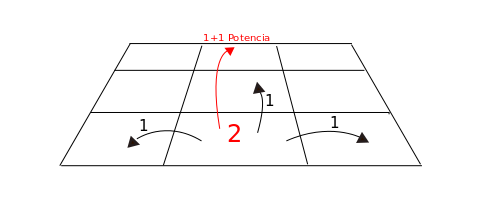
\includegraphics[scale=0.9]{images/saltos}
\end{center}
El objetivo del juego es llegar de una celda origen a otra destino, realizando la menor cantidad de saltos posibles. Por esto, se pide el diseno e implementaci\'on de un algoritmo que calcule y de como resultado uno de los caminos que lleguen de origen a destino cuya cantidad de saltos sea m\'inima.
\vspace{2mm}


El algoritmo tiene que tener una complejidad de $O(n^3*k)$, con $n$ la cantidad de filas y columnas del campo de juego y $k$ la cantidad de potencias otorgadas al inicio del juego al jugador.
\vspace{2mm}
\subsection{Ideas para la resoluci\'on} \label{ej_3:idea}

Decidimos encarar la resolucio\'on como un problema de grafos. El campo de juego es representado como un grafo con un nodo por cada celda, y las aristas son orientadas, de peso constante y representan todos los posibles saltos entre celda y celda. 
\begin{center}
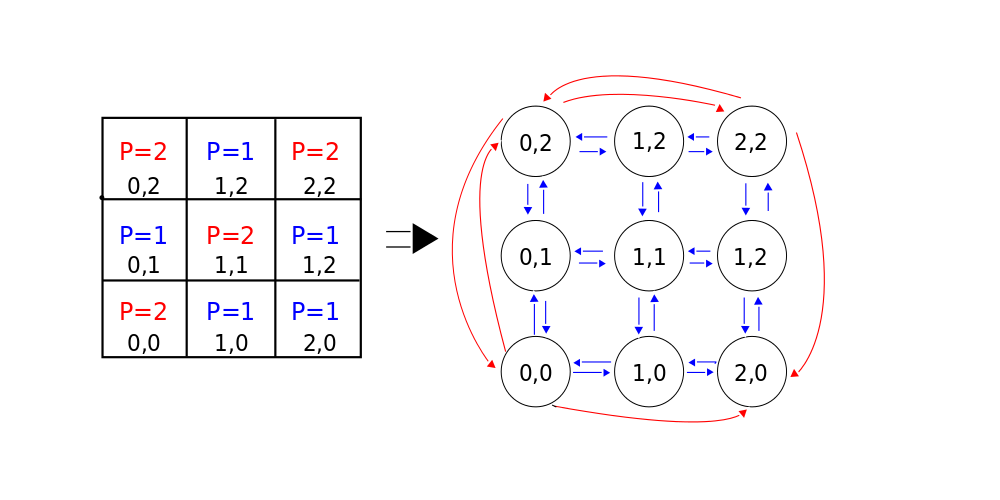
\includegraphics[scale=0.5]{images/grafo1}
\end{center}
\vspace{2mm}


Por cada uno de los valores $0..k$ de potencia tenemos un campo de juego de los anteriormente mencionados. Los vamos a llamar $"niveles"$, y van a ser subgrafos interconectados para formar un grafo general que va a resolver el problema. Entre estos niveles va a haber aristas conectando los nodos de mayor nivel con los de menor nivel, representando el hecho de $"gastar"$ potencias, es decir, si en un turno estoy en el nivel $k$ y utilizo dos potencias, en el siguiente turno voy a estar posicionado en un nodo del nivel $k-2$.

\vspace{2mm}

De esta forma, estar en el nodo $(i,j)$ del nivel $k$ representa estar posicionado en la celda de juego $(i,j)$ y disponer de $k$ potencias para utilizar .Podemos $"saltar \: entre \: celdas"$, movi\'endonos de un nodo a otro usando las aristas este nivel. En caso de querer usar las potencias, debemos movernos por aristas que conectan los nodos de nivel $k$ con los niveles inferiores. Por ejemplo, si estamos en el nodo $(i,j,k)$, de potencia 2, y queremos saltar 3 nodos hacia la derecha, debemos tomar la arista orientada que nos lleva al nodo $(i+3,j,k-1)$ (en caso de disponer de una potencia). De esto deducimos que las aristas entre niveles s\'olo salen de nodos de nivel superior hacia nodos de nivel inferior. Formalicemos esto:

\vspace{2mm}

Para cada nivel, sea:

\begin{align*}
G_L = (V_L, E_L) /\: V_ = {V_{1_{L}},..., V_{n_{L}}} =  \{ casillas \: 1..n  \:con \: L \: potencias \: disponibles \}
\end{align*}
\vspace{2mm}
Por lo tanto, el grafo $G$ es:

\begin{align*}
G = (W, A) /\: W \: =  \:\cup_{i=1}^{k} V_i(G_i) \: \land \: A \: = \: (\cup_{L=1}^{k} E_L(G_L)) \cup T
\end{align*}

\vspace{2mm}

Donde $T$ son las aristas entre niveles, descriptas a continuaci\'on:

\vspace{2mm}

Se tienen aristas dirigidas en cada nivel tal que si $v, u \in V_t$, $(u,v) \in E_t$ sii $v$ es alcanzable desde $u$ sin usar potencias.
Dados niveles $G_m,\, G_j\, /\, m\,< \,j$ y dos v\'ertices $v \in V_m(G_m) \: \land \: w \in V_j(G_J)$ existe una arista dirigida $"entre"$ niveles, que pertenezca a $T$, sii $w$ es alcanzable desde $v$ usando estrictamente $(j-m)$ unidades de potencia, es decir, que la distancia en casillas (verticales u horizontales) de $v$ a $w$ es igual a $(j-m) + pot(v)$.

\vspace{2mm}

En el siguiente diagrama mostramos las aristas entre niveles que deber\'ian tomarse en caso de usar una potencia en las celdas $(0,2)$ y $(2,0)$

\begin{center}
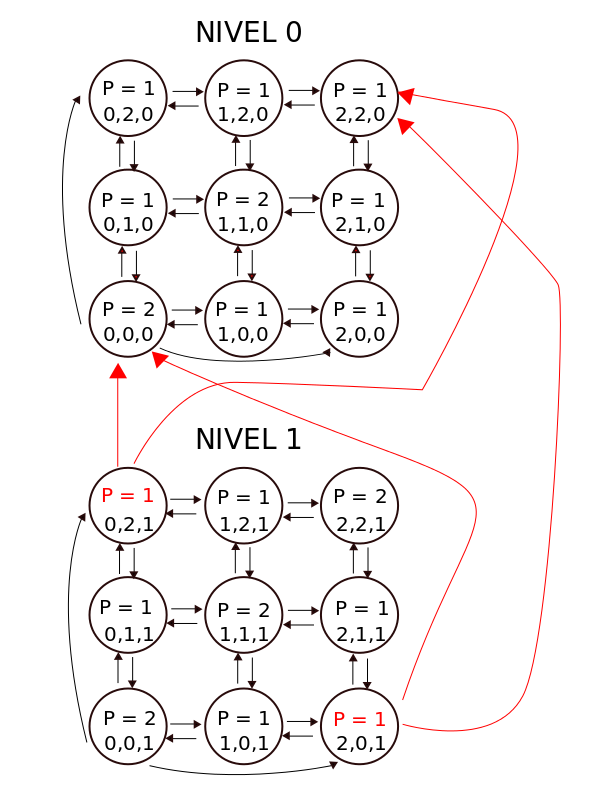
\includegraphics[scale=0.5]{images/dospisos}
\end{center}
\vspace{2mm}

Notemos que al avanzar hacia niveles m\'as bajos no se puede ir hacia arriba (lo cual tiene sentido pues el nivel actual indica la cantidad de potencias disponibles para usar, y este valor nunca puede aumentar)

\vspace{2mm}

Definimos $n_0$ como el nodo origen $/ n_0 \in V_k$ (primer nivel, m\'as alto), dado por las coordenadas cartesianas de la celda de comienzo de la entrada. Si la celda destino en el juego es $(i,j)$ definimos el conjunto de nodos destino como los nodos $(i,j,k)$, con $k$ entre 0 y la cantidad de potencias m\'axima, de forma que al llegar al nodo destino $(i,j,l)$, l es la cantidad de potencias sin usar.

\vspace{2mm}

Las aristas son de peso constante en su totalidad (en particular, 1). Adem\'as, en cada arista se guarda un valor indicando la cantidad de niveles atravesadas en este paso, lo cual es equivalente a la cantidad de potencias utilizadas en el salto. No confundir este valor con el costo o peso de la arista.
\vspace{2mm}
(Dibujo zarpado)
\vspace{2mm}

De esta forma, encontrar el camino que realize la menor cantidad de saltos se reduce a buscar el camino m\'as corto en el grafo de $n_0$ a alg\'un nodo destino, guardando en cada caso el valor de cada arista (potencia usada) y la posici\'on $(i,j)$ del nodo sin importar el nivel actual. Un recorrido de anchura BFS del grafo nos brinda el camino m\'as corto, comenzando la b\'usqueda desde $n_0$.

\subsection{Estructuras de datos}

A cada una de las celdas, las representamos con la clase $nodo$, que posee tres atributos: $x$, $y$ y $level$, (el numero de fila y columna de la celda que representa este nodo, y el nivel en el que se encuentra el nodo).

\vspace{2mm}

Representamos el grafo en memoria con una modificaci\'on del m\'etodo de listas de adyacencia. La estructura es un diccionario (java $HashMap$) llamado graph, cuyas claves son los nodos y sus definiciones son el tipo $NodoMetadata$.

\vspace{2mm}

La clase $NodoMetadata$ brinda la informaci\'on necesaria de cada nodo para poder armar el grafo, ya que contiene el atributo $alcanzables$, que es su lista de adyacencia. Adem\'as de esto, posee tres atributos m\'as: $nodoValue$, $fueVisitado$ y $predecesor$, el primero representando la potencia del resorte de la celda, y los otros dos son de utilidad al bfs, para $"marcar"$ un nodo, e indicar su antecesor en el recorrido de \'este.

\vspace{2mm}

Finalmente tenemos una clase $Juego$ que unifica todo, cuyos atributos son un nodo inicial, un nodo destino, y el diccionario graph.



\subsection{Algoritmos y Complejidad} \label{ej_3:algoritmo}
El algoritmo consta de varias etapas principales:
\begin{enumerate}
	\item Generaci\'on del grafo a partir de los datos de entrada.
	\item Busqueda del camino m\'inimo(en cantidad de pasos) con un BFS.
	\item Construcci\'on del camino a trav\'es de los predecesores del destino indicados por BFS y
 			c\'alculo de potencia utilizado en cada salto.
 \end{enumerate}

 \subsubsection{Generaci\'on del Grafo}

A continuaci\'on mostramos un pseudoc\'odigo de la generaci\'on del juego. Durante las demostraciones, se usar\'a la variable $k$ para referirse a la cantidad de potencias iniciales al iniciar el juego, y la variable $n$ como la cantidad de filas del juego.
\vspace{2mm}
\begin{algorithmic}[1]
\Statex
	\Procedure{Juego}{$int[\,][\,] valores, int\, potInicial, int \,filInicial, \,int colInicial,  int\, filDestino, int \,colDestino$}
	\State $Juego.nodoInicial \gets new \: Nodo(filInicial, colInicial, potInicial)$
	\Comment{$O(1)$}
	\State $Juego.nodoDestino \gets new \: Nodo(filDestino, colDestino, 0) $
	\Comment{$O(1)$}
	\State $Juego.graph \gets new \: HashMap<Nodo,\: NodoMetadata>()$
	\Comment{$O(1)$}
	\State $int \: dimension \gets longitud(valores)$
	\Comment{$O(1)$}
	\For{$int\:  level \gets potInicial;\: level \geq 0;level--$}
	\Comment{$O(potInicial)$}
		\For{$int \: i \gets 0;\: i\,<\,dimension;\:i++$}
		\Comment{$O(dimension)$}
			\For{$int  \:j\gets 0; \:j<dimension; \:j++$}	
			\Comment{$O(dimension)$}
				\State	$Nodo \: nodo\gets new \: Nodo(i,\: j,\: level)$
				\Comment{$O(1)$}
				\State	$int\: nodoValue \gets valoress[i][j]$
				\Comment{$O(1)$}
				\If{$nodoValue>dimension$}
					\State $nodoValue \gets dimension$
				\EndIf
				\State	$boolean \:fueVisitado \gets false$
				\Comment{$O(1)$}
				\State	$List<Nodo>:, alcanzables \gets calcularAlcanzables(nodo,\, nodoValue,\, dimension)$
				\Comment{$O(dimension)$}
				\State	$NodoMetadata \, metaData \gets new\, NodoMetadata(nodoValue,\, fueVisitado,\, alcanzables,\, null)$
				\Comment{$O(1)$}
				\State	$graph.put(nodo,\: metaData)$
				\Comment{$O(1)$}
			\EndFor
		\EndFor
	\EndFor

\EndProcedure
\Statex
\end{algorithmic}
\vspace{2mm}

Donde valores representa la matriz de celdas con sus respectivas potencias de resorte, potInicial representa $k$, la cantidad de potencias que se le brinda a un jugador al iniciar el juego, y $filInicial$, $colInicial$, $filDestino$, $colDestino$ las coordenadas respectivas de la celda de inicio y la celda destino. Cabe aclarar, en la l\'inea 11, en caso de que en la entrada, una celda posea un valor de resorte mayor a la dimensi\'on del campo de juego, fijamos el valor del nodo como $dimension$, ya que no tiene sentido poseer un resorte que permita saltar fuera de los l\'mites de la matriz, es decir, el jugador s\'olo va a poder usar uso de la potencia del resorte como m\'aximo hasta el valor dimensi\'on. Esto nos permite ajustar el c\'alculo de complejidad de la funci\'on siguiente.

\vspace{2mm}

Complejidad:

Los 3 ciclos for anidados indican una complejidad de $O(k*n^2)$. Dentro de estos ciclos se realizan operaciones, todas de tiempo constante $O(1)$ excepto la llamada a a funci\'on $alcanzables$, que toma $O(n)$, y ser\'a justificado a continuaci\'on, d\'andonos un total de $O(k*n^3)$ en la construccion del grafo para nuestro modelo.

\vspace{10mm}		

 \subsubsection{C\'alculo de alcanzables}

Funci\'on auxiliar que para un nodo, calcula todos los otros nodos a los que podri\'a $"saltar"$, usando y no usando potencias. La salida del algoritmo es del tipo $Lista<Nodo>$.
\vspace{2mm}
\begin{algorithmic}[1]
\Procedure{calcularAlcanzables}{$Nodo\: nodo,\:int\: valorNodo,\: int \:dimension$}
		\State $int\: nivelActual\: =\: nodo.getLevel()$
		\Comment{$O(1)$}
		\State $int\: actualX\: =\: nodo.getX()$
		\Comment{$O(1)$}
		\State $int\: actualY\: =\: nodo.getY()$
		\Comment{$O(1)$}
		\State $int\: resorte\: =\: valorNodo$
		\Comment{$O(1)$}
		\State $Lista<Nodo>\: alcanzables\: =\: new\: Lista<Nodo>$
		\Comment{$O(1)$}
		\For{$int\: j \gets -resorte;\:j\leq resorte;\:j++$}
		\Comment{$O(resorte)\: acotado \: por \: O(dimension)$}
			\If{$validarBordes(dimension,\: actualX,\: j)$}
			\Comment{$O(1)$}
				\State $Nodo\: alcanzableDir\gets new\: Nodo(actualX\: +\: j,\: actualY, \:nivelActual)$
				\Comment{$O(1)$}
				\State $alcanzables.agregar(alcanzableDir)$
				\Comment{$O(1)$}
			\EndIf
				
			\If{$validarBordes(dimension,\: actualY,\: j)$}
			\Comment{$O(1)$}
				\State $Nodo\: alcanzableDir \gets new \:Nodo(actualX, \:actualY\: + \:j, \:nivelActual)$
				\Comment{$O(1)$}
				\State $alcanzables.agregar(alcanzableDir);$
				\Comment{$O(1)$}
			\EndIf
		\EndFor

		\For{$int\: potAdic\gets 1;\:potAdic+\leq nivelActual;\:potAdic++$}
			\Comment{$O(dimension)$}
			\State $int\: potTotal \gets potencia\: +\: potAdic; $
			\If{$potTotal>dimension$}
				\State $break$
			\EndIf
			\If{$validarBordes(dimension, \:actualY,\: potTotal)$}
			\Comment{$O(1)$}
				\State $Nodo\: alcanzableIndir = new\: Nodo(actualX,\: actualY +\: potTotal, \:nivelActual - \:potAdic)$
				\Comment{$O(1)$}
				\State $alcanzables.agregar(alcanzableIndir)$
				\Comment{$O(1)$}
			\EndIf

			\If{$validarBordes(dimension, \:actualY,\: -potTotal)$}
			\Comment{$O(1)$}
				\State $Nodo\: alcanzableIndir = new\: Nodo(actualX,\: actualY -\: potTotal, \:nivelActual - \:potAdic)$
				\Comment{$O(1)$}
				\State $alcanzables.agregar(alcanzableIndir)$
				\Comment{$O(1)$}
			\EndIf

			\If{$validarBordes(dimension, \:actualX,\: potTotal)$}
			\Comment{$O(1)$}
				\State $Nodo\: alcanzableIndir = new\: Nodo(actualX  +\: potTotal,\: actualY, \:nivelActual - \:potAdic)$
				\Comment{$O(1)$}
				\State $alcanzables.agregar(alcanzableIndir)$
				\Comment{$O(1)$}
			\EndIf

			\If{$validarBordes(dimension, \:actualX,\: -potTotal)$}
			\Comment{$O(1)$}
				\State $Nodo\: alcanzableIndir = new\: Nodo(actualX  -\: potTotal,\: actualY, \:nivelActual - \:potAdic)$
				\Comment{$O(1)$}
				\State $alcanzables.agregar(alcanzableIndir)$
				\Comment{$O(1)$}
			\EndIf

		\EndFor	
		\State $return alcanzables$
		\Comment{$O(1)$}
\vspace{2mm}
\EndProcedure
\end{algorithmic}

\vspace{2mm}

Donde $nodo$ es el nodo del cual se van a calcular sus alcanzables, $valorNodo$ la potencia de su resorte y dimension es $n$. Podemos ver que al algoritmo lo componen dos ciclos for lineales, que van armando la lista $alcanzables$. El primer ciclo, calcula los nodos alcanzables $Directos$, es decir, aquellos a los que puede saltar con el resorte de la celda sin hacer uso de ninguna potencia adicional.El ciclo itera de $-resorte$ a $resorte$, agregando de \'esta forma a la lista de alcanzables los nodos a su izquierda, derecha, hacia adelante y atr\'as, validando con cuidado los bordes de la matriz, y sin agregarse a s\'i mismo, tomando cada uno de estos pasos $(O(1))$. Dado que la potencia de un resorte est\'a acotada por la dimensi\'on de la matriz (por la forma en la que generamos el grafo), este ciclo itera como m\'aximo de $-dimension$ a $dimension$, por lo tanto $\in O(n)$. 

\vspace{2mm}

El segundo ciclo for calcula todos los nodos alcanzables indirectamente, es decir, aquellos para los cuales el jugador tiene que 1 o m\'as de sus potencias extra para poder llegar. Este ciclo itera segu\'un la variabie $potAdic$, potencias adicionales, que comienza en 1 hasta el nivel del nodo en cuesti\'on (recordar que el nivel de un nodo representa la cantidad de potencias extra que le quedan a un jugador). Este valor se le suma a la potencia del resorte (l\'inea 18) y si se validan bien los bordes, se agregan estos nodos ($O(1)$), los que est\'an a distancia $potencia \: de \: resorte + \: potAdic$, y al iterar $potAdic$ hasta el nivel del nodo obtenemos todos los nodos alcanzables usando las potencias que le quedan disponibles al jugador. Estas acciones se realizan en $O(1)$, y el ciclo itera de 1 hasta el nivel del nodo.

\vspace{2mm}

 Esto indicar\'ia que el ciclo tendr\'ia una complejidad de $O(k)$, por ser $k$ el nivel m\'aximo del grafo, pero podemos acotar esto, en la l\'inea 19, por el mismo motivo que en el ciclo anterior, una vez que la potencia total a usar supera el valor de la dimensi\'on de la matriz, cortamos el ciclo, ya que no tiene sentido saltar fuera del campo de juego. Por lo tanto calculamos para los posibles valores de potencia adicional que le queden al jugador, hasta que la potencia total de salto sea de $dimension$. Por lo tanto el ciclo tambi\'en $\in O(dimension)$. Como comentario adicional, remarcamos que es posible agregar este condicional a la guarda del ciclo, pero dada la complejidad de entendimiento de este pseudoc\'odigo decidimos ponerlo como una instrucci\'on de $break$ para mayor claridad.

 \vspace{2mm}

Concluimos en que la funci\'on tiene una complejidad de $O(n) + O(n)$ = $O(n)$. Lo cual tiene sentido, ya que si consideramos la matriz de juego, un nodo como m\'aximo puede moverse hacia todos los de su fila y columna, es decir a $2n - 2$ nodos, lo cual concuerda con la complejidad ya que anadimos cada uno de ellos a la lista de alcanzables en tiempo constante.

\subsubsection{B\'usqueda del camino m\'inimo}

A continuaci\'on el pseudoc\'odigo de la b\'usqueda BFS. Se trata de una modificacion de BFS que busca un camino entre el nodo inicial y alguno de los nodos destino, sin importar a qu\'e nivel pertenezcan, es decir, cuando la b\'usqueda encuentra un nodo w tal que las primeras 2 coordenadas de w coinciden con la celda destino, termina el algoritmo. Acto seguido reconstruye el camino en base a los predecesores, que se van guardando a medida que se realiza la expansion en anchura. Teniendo en cuenta que BFS encuentra el camino mas corto en cantidad de aristas entre 2 nodos, esto resuelve nuestro problema. La salida es una lista de nodos que comprende el camino, indicando en cada paso: (posX, posY, gasto de PowerUp en el salto del predecesor de este nodo al actual).

\vspace{2mm}
\begin{algorithmic}[1]
\Procedure{caminoMinimo}{$Juego j$}{$List<Nodo>$}

	\State$Cola<Nodo>\: cola \gets new \:Cola<Nodo>$
	\Comment{$O(1)$}
	\State$cola.encolar(nodoInicial)$
	\Comment{$O(1)$}
	\State$marcarVisitado(nodoInicial)$
	\Comment{$O(1)$}
	
	\While{$\neg cola.esVacia()$}
	\Comment{$O(dimension^2)$}
		\State $Nodo \:actual \gets cola.desencolar()$
		\Comment{$O(1)$}
		\If{$esDestino(actual)$}
		\Comment{$O(1)$}
			\State $return \: construirCaminoConPredecesores(actual)$
			\Comment{$O(dimension^2*potInicial)$}

		\EndIf
			
		\State $Lista<Nodo> \: alcanzables \gets obtenerAlcanzables(actual)$
		\Comment{$O(dimension)$}
		\ForAll{$Nodo\: alcanzable : alcanzables$}
		\Comment{$O(dimension)$}
			\If{$\neg estaVisitado(alcanzable)$}
			\Comment				
				\State$marcarVisitado(alcanzable)$
				\Comment{$O(1)$}
				\State$	asignarPredecesor(alcanzable,\: actual)$
				\Comment{$O(1)$}
				\State$	cola.encolar(alcanzable)$	
				\Comment{$O(1)$}			
			\EndIf
			
		\EndFor
		\EndWhile
		\State $return\: null$
		\Comment{$O(1)$}

\EndProcedure
\end{algorithmic}
\vspace{2mm}

	Podemos ver que el c\'odigo es an\'alogo al de el algoritmo BFS, con el agregado de que adem\'as de marcar cada nodo $i$ una vez visitado, se le asigna un predecesor $j$, que es el nodo para el cual $i$ pertenece a la lista de alcanzables de $j$, en el orden de la b\'usqueda. De esta forma, cuando encuentra al nodo $destino$, puede reconstruir el camino que realiz\'o la b\'usqueda visitando todos los precedesores hasta llegar al nodo $origen$, de lo cual se encarga la pr\'oxima funcio\'on.

\vspace{2mm}

	El while principal del ciclo recorre todos los nodos en el peor caso (cuando la b\'usqueda no se detiene en la l\'inea 7. En cada iteraci\'on, se visita un nodo, se lo marca para no visitarlo nuevamente, y se verifica que no sea el nodo que estamos buscando(nodo destino).
	Si lo es, termina el algoritmo de b\'usqueda y se llama a la funci\'on $construirCaminoConPredecesores$. Caso contrario, se agregan a la cola todos los nodos adyacentes(alcanzables) no visitados, ademas se indicar para cada uno de ellos que el nodo anterior es su predecesor

	\vspace{2mm}

	Obtener los adyacentes de un nodo se realiza en tiempo constante $O(1)$ (acceder al hashmap por clave) y $O(n)$ para encolar todos los adyacentes (anteriormente argumentado). Sea $f(G, i)$ = {cantidad de nodos sin visitar en G en la iteracion i}, esta funcion tiene un valor inicial $f(G,\: 0)$ = $n^2*k$ y en cada iteracion esta funcion decrece y toma el valor cero en $f(G, \:n^2*k)$ = $f(G,\: cantNodosG)$ = $0$. En este momento, no hay mas nodos no visitados para agregar a la cola. Luego, se procesar\'an todos los elementos encolados y terminar\'a el algoritmo.
	\vspace{2mm}


	 Juntando todas estas observaciones vemos que el $while(!queue.isEmpty())$ est\'a asociado a la funci\'on $f(G,\: i)$, que decrece en cada iteraci\'on al menos una unidad, en el peor de los casos, tomara $O(f(G,\:0))$ = $O(n^2*k)$ = $cantNodos \:de\: G \:al\: comenzar$ en recorrer todos los nodos. La funci\'on esDestino(...) toma tiempo constante, de ingresar en este if, termina el algoritmo con un costo $O(f(G,\: 0))$ adicional por armar	el camino con la funcion $construirCaminoConPredecesores$. La lista de alcanzables se obtiene en $O(1)$, iterar sobre los alcanzables realizando operaciones de tiempo constante dentro de este subciclo toma $O(n)$. En total, este metodo tiene una complejidad temporal: iterar sobre todos los nodos y fijarse si es destino: $O(k*n^2))*(O(1))$, obtener nodos alcanzables: $O(1)$, encolar lcanzables: $O(n)$ y al finalizar armar el camino: $O(k*n^2)$	= $O(k*n^2)*O(n) + O(k*n^2) = O(k*n^3) $.

\vspace{2mm}

 \subsubsection{Construcci\'on del camino}

Finalmente, el pseudoc\'odigo de la funci\'on que genera el camino a partir del recorrido que realiz\'o el BFS. La salida del algoritmo es del tipo $Lista<Nodo>$.
\vspace{2mm}
\begin{algorithmic}[1]
\Procedure{construirCaminoConPredecesores}{$Nodo \: actual$}


		\State $Lista<Nodo>\: camino \gets new\: Lista<Nodo>$
		\Comment{$O(1)$}	
		\State $Nodo\: nodo \gets actual$
		\Comment{$O(1)$}	
		\While{$damePredecesor(nodo) != null)$}
		\Comment{$O(dimension*dimension)$}	
			\State $Nodo\: predecesor \gets damePredecesor(nodo)$
			\Comment{$O(1)$}	
			\State $nodo.nivel \gets predecesor.nivel()\: -\: nodo.nivel()$
			\Comment{$O(1)$}	
			\State $camino.agregarAdelante(nodo)$
			\Comment{$O(1)$}	
			\State $nodo \gets predecesor$
			\Comment{$O(1)$}	

		\EndWhile

		\State $nodo.setLevel(0)$
		\Comment{$O(1)$}	
		\State $camino.agregarAdelante(nodo)$
		\Comment{$O(1)$}	
		\State $return\: camino$
		\Comment{$O(1)$}	
		
\EndProcedure
\end{algorithmic}

La lista de nodos del camino va a ser a lo sumo $n^2$, dandonos una complejidad de $O(n^2)$ dado que el ciclo que arma el camino itera una vez por cada nodo en base a los predecesores. Adentro del ciclo se realizan operaciones de tiempo constante, dandonos una complejidad temporal total de $O(n^2)$.

\vspace{2mm}

Dado que el algoritmo BFS nos brinda el camino m\'as corto en aristas de el nodo origen al destino, llegamos a la conclusi\'on de que la complejidad depende de $n^2$, que es la cantidad de nodos, ya que como m\'aximo va a visitar cada uno de los $k$ nodos $(i,j,0..k)$ una \'unica vez. Supongamos que esto no ocurre, y el camino m\'inimo visita al menos dos nodos $(i,j,k_1)$ y $(i,j,k_2)$. Si volvemos a pensar el grafo como el tablero de juego bidimensional, estar\'ia volviendo a la misma celda otra vez, s\'olo que con menos unidades de potencia (de ah\'i la diferenciad de nivel), formando un ciclo, el cual podr\'iamos retirar para quedarnos con un camino m\'as corto. Esto es absurdo, ya que consideramos m\'inimo el anterior camino, por lo tanto, el camino m\'inimo va a visitar como m\'aximo una vez cada celda, la complejidad va a ser $O(n^2)$.
 
 \subsubsection{Complejidad Total}

 Complejidad total:
\begin{enumerate}

\item Armar el grafo: $O(k*n^3)$
\item Algoritmo de busqueda en anchura y armado del camino: $O(k*n^3)$
 \end{enumerate}
\vspace{2mm}
 Por lo tanto la complejidad es $O(k*n^3)$ como lo pide el enunciado.

\vspace{2mm}

Documentaci\'on de la clase HashMap:

 http://docs.oracle.com/javase/7/docs/api/java/util/HashMap.html



\subsection{Casos de prueba y resultado del programa} \label{ej_3:casos}

Compilador GJC: Java realiza un profiling sobre el programa a compilar y toma estadisticas para realizar diferentes procesos de compilacion/interpretacion sobre el codigo, esto se ve reflejado en el tiempo de ejecucion del programa compilado con el jdk, para forzar la compilacion de java a codigo objeto, utilizamos el compilador GCJ de GNU, que es uno de los compiladores denominados Ahead-Of-Time. Todos los experimentos fueron ejecutados sobre el programa compilado a codigo nativo. La cantidad de iteraciones por cada entrada es 100 para licuar los posibles outliers.

\vspace{2mm}

Interpretacion de los graficos: Como se puede ver en los graficos, la complejidad empirica, coincide con la complejidad teorica esperada $O(k*n^3)$, llegamos a esta conclusion graficando los siguientes casos: $k$ = $[0..5]$ $n$ = $[2..100]$ para cada caso, se realizaron 3 graficos, $(X,F(X))$,  $(X,F(X)/x^2)$ y $(X,F(X)/x^3)$. En estos graficos se puede observar que al dividir por $x^2$ se obtiene una curva con crecimiento lineal aproximado, y al dividir por $x^3$, se obtiene una constante aproximada, es decir, una curva acotada entre una diferencia pequena en el eje X, concluyendo que la curva inicial corresponde a una funcion $f(n)$ = $q.n^3$, con $q$ en $R$. Asimismo veamos que cuando se incrementa el valor de $k$ para los graficos anteriores, la imagen de las funciones graficadas crecen linealmente a medida que crece $k$. Lo que nos indica que en realidad las funciones graficadas son realmente $f(n)$ = $j.(k.n^3)$, con $j$ en $R$, concluyendo, $f(n)$ $\in$ $O(k*n^3)$. Referencia: http://www.excelsior-usa.com/jetcs00007.html

\vspace{2mm}

Con k = 0

\begin{center}
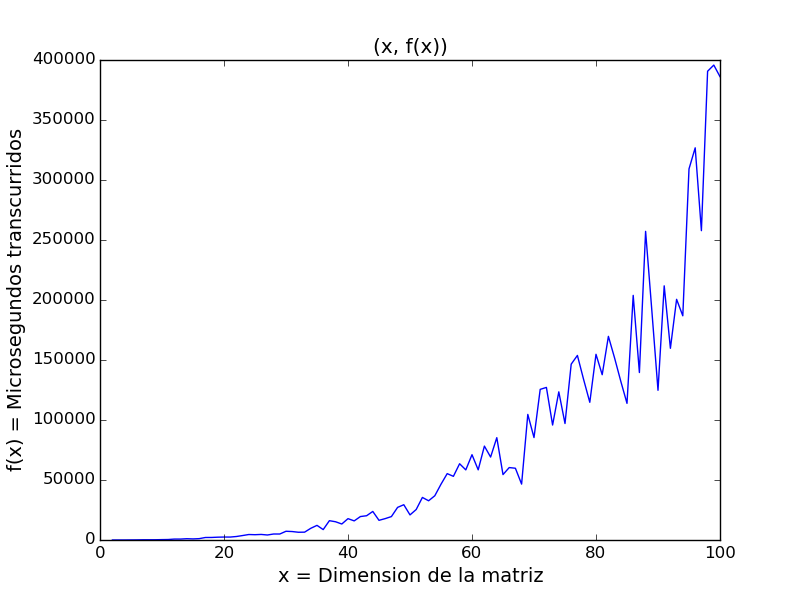
\includegraphics[scale=0.54]{images/0potenciafuncion}
\end{center}


\begin{center}
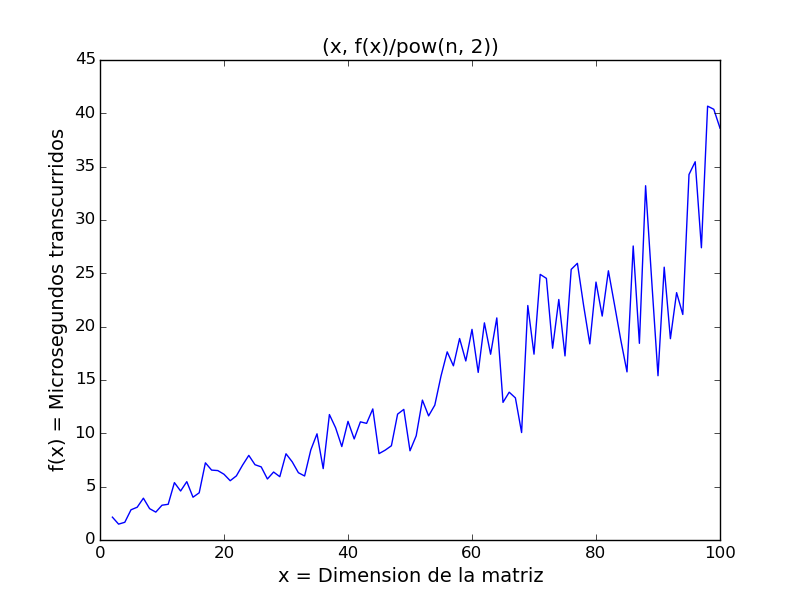
\includegraphics[scale=0.54]{images/0potenciasobrecuadrado}
\end{center}


\begin{center}
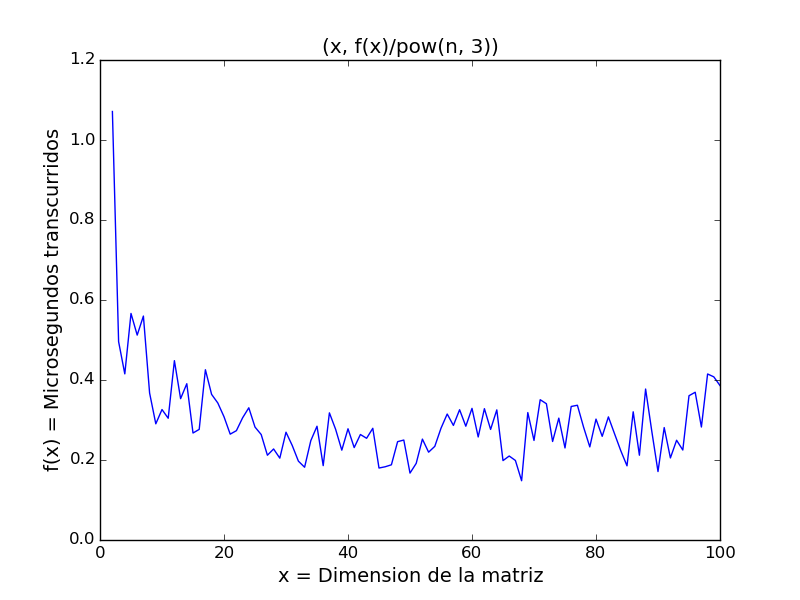
\includegraphics[scale=0.54]{images/0potenciasobrecubo}
\end{center}
\vspace{2mm}
\vspace{2mm}
\vspace{2mm}

Con k = 1

\begin{center}
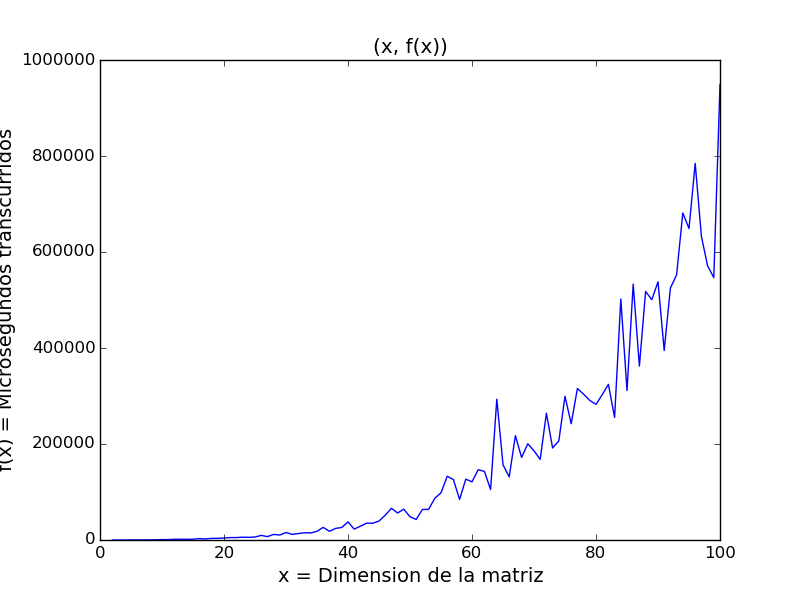
\includegraphics[scale=0.54]{images/1potenciafuncion}
\end{center}


\begin{center}
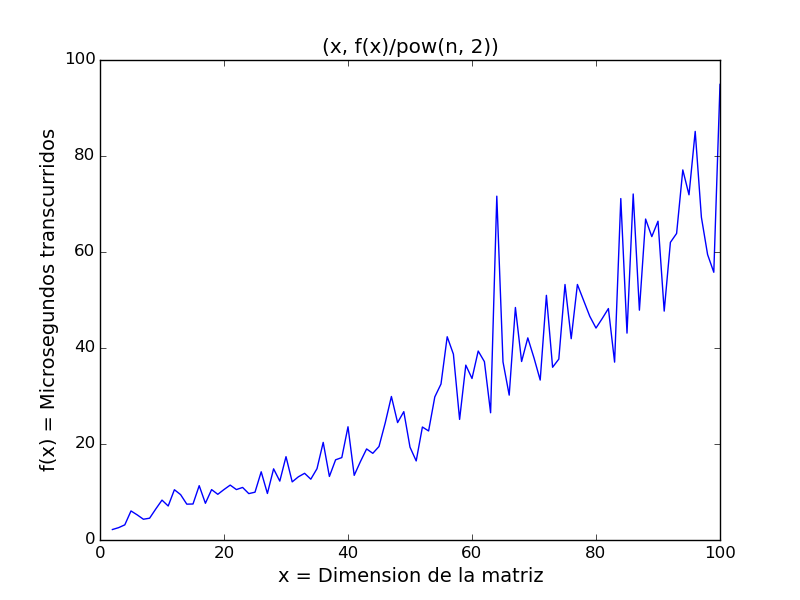
\includegraphics[scale=0.54]{images/1potenciasobrecuadrado}
\end{center}


\begin{center}
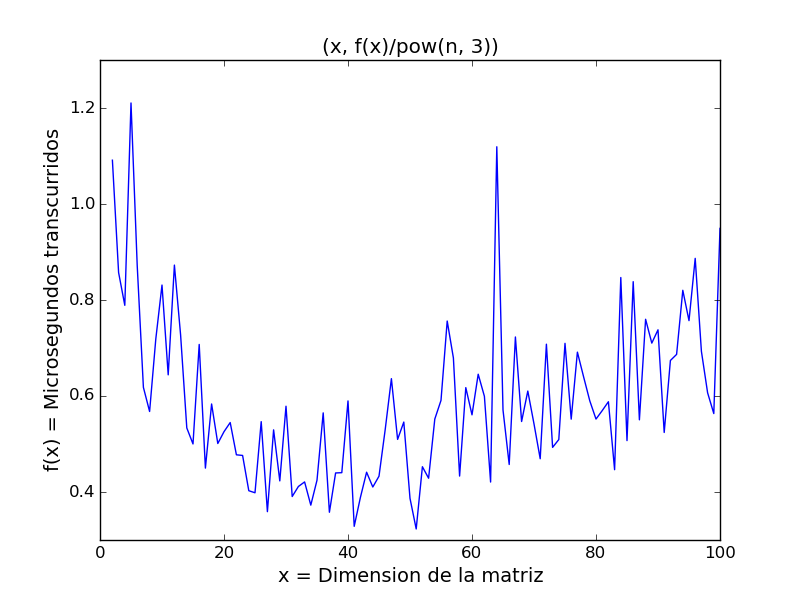
\includegraphics[scale=0.54]{images/1potenciasobrecubo}
\end{center}


\vspace{2mm}

Con k = 2


\begin{center}
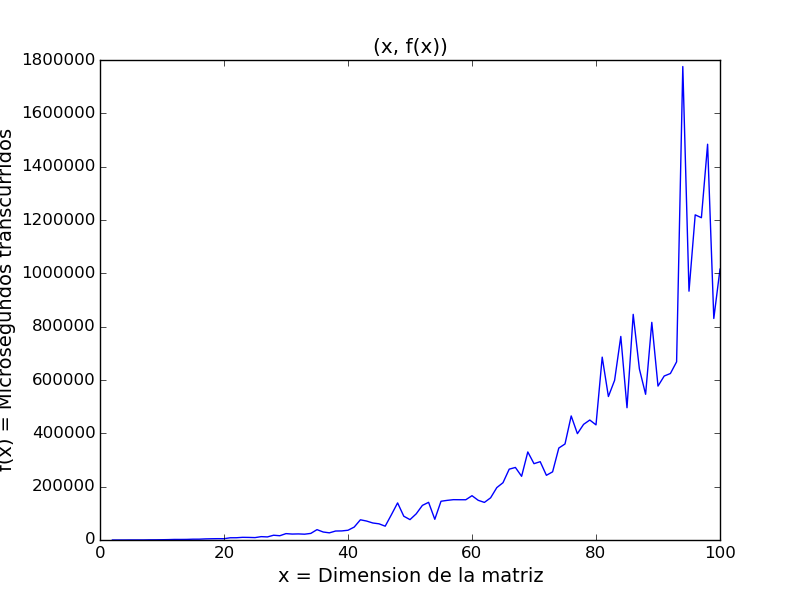
\includegraphics[scale=0.54]{images/2potenciafuncion}
\end{center}


\begin{center}
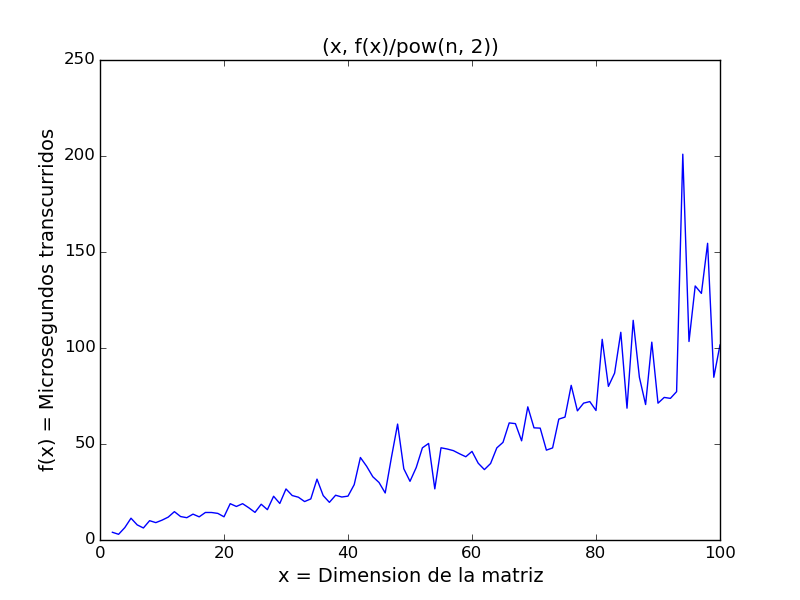
\includegraphics[scale=0.54]{images/2potenciasobrecuadrado}
\end{center}


\begin{center}
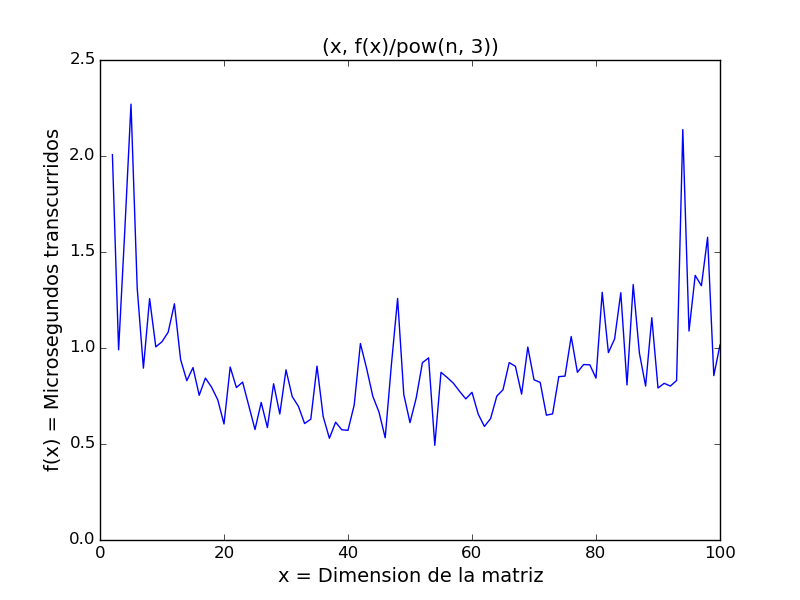
\includegraphics[scale=0.54]{images/2potenciasobrecubo}
\end{center}


\vspace{2mm}

Con k = 3


\begin{center}
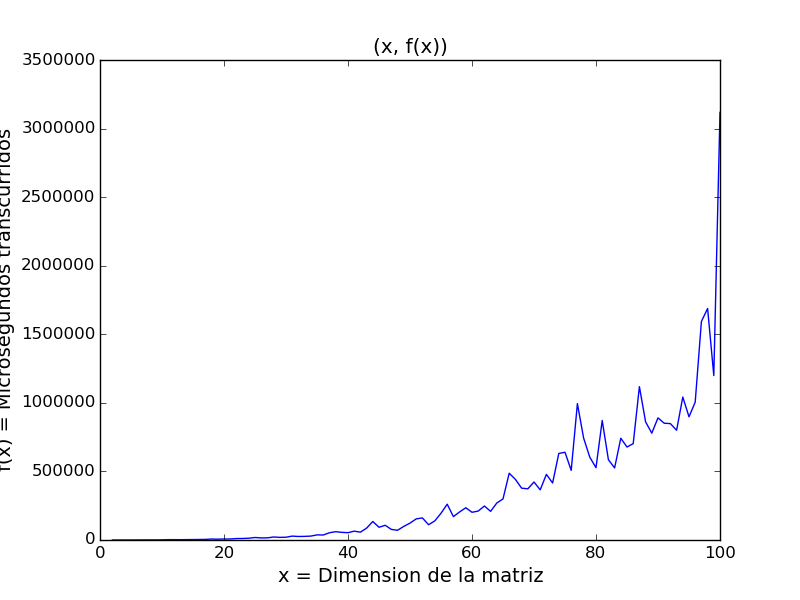
\includegraphics[scale=0.54]{images/3potenciafuncion}
\end{center}


\begin{center}
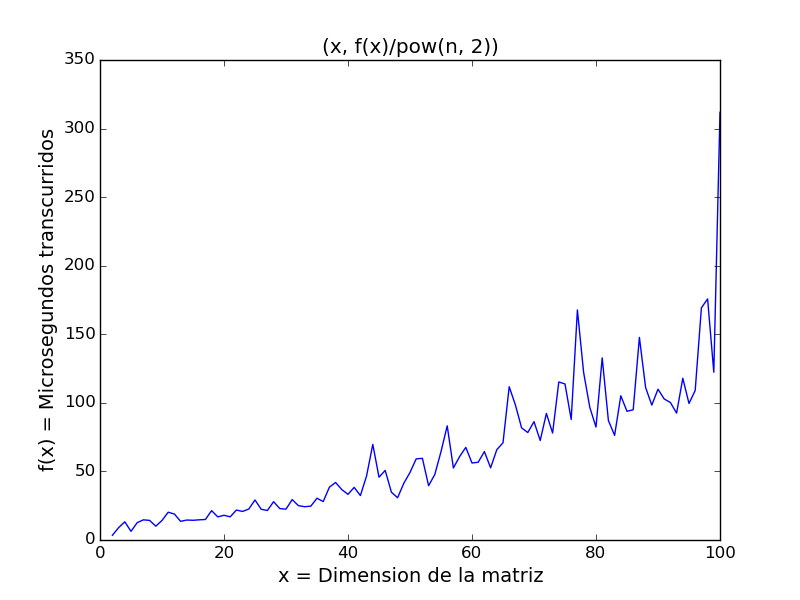
\includegraphics[scale=0.54]{images/3potenciasobrecuadrado}
\end{center}


\begin{center}
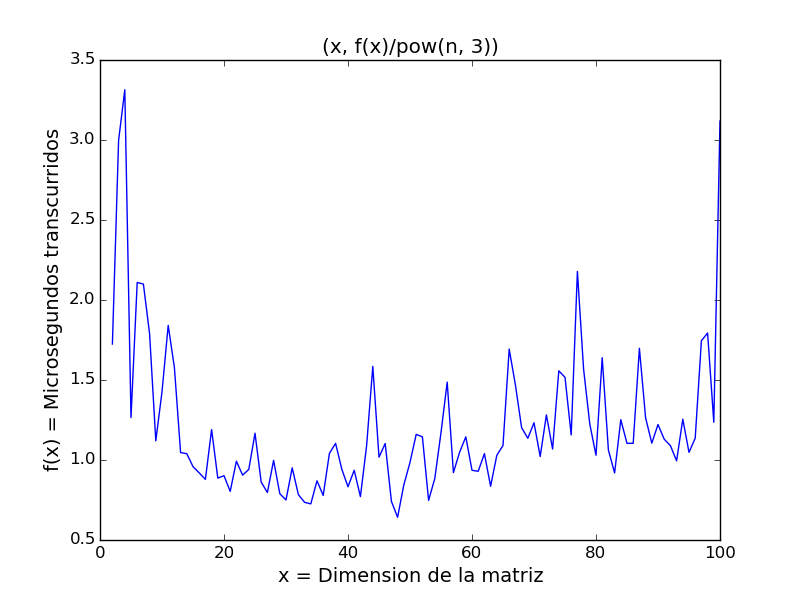
\includegraphics[scale=0.54]{images/3potenciasobrecubo}
\end{center}


\vspace{2mm}

Con k = 4


\begin{center}
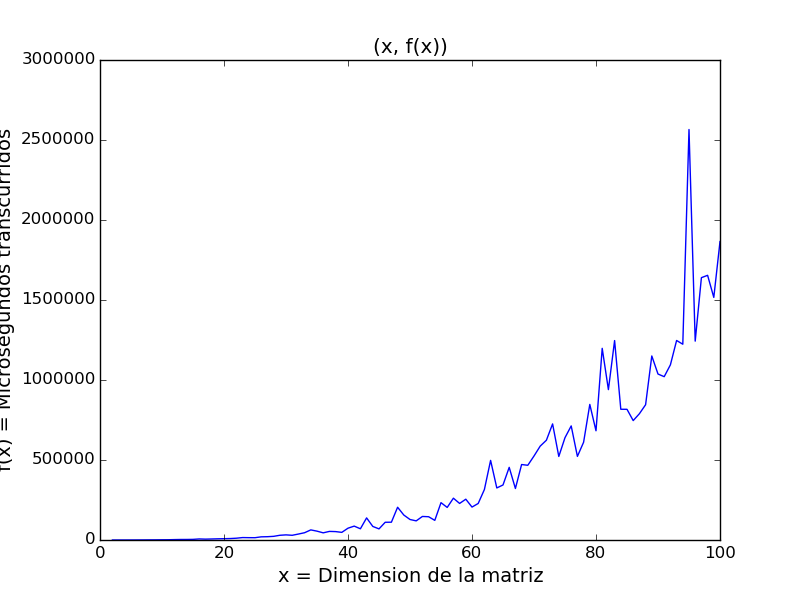
\includegraphics[scale=0.54]{images/4potenciafuncion}
\end{center}


\begin{center}
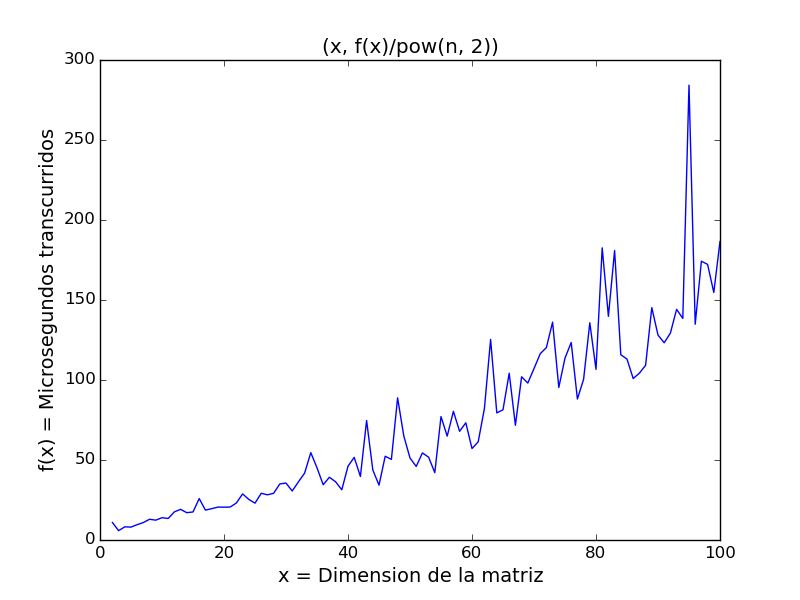
\includegraphics[scale=0.54]{images/4potenciasobrecuadrado}
\end{center}


\begin{center}
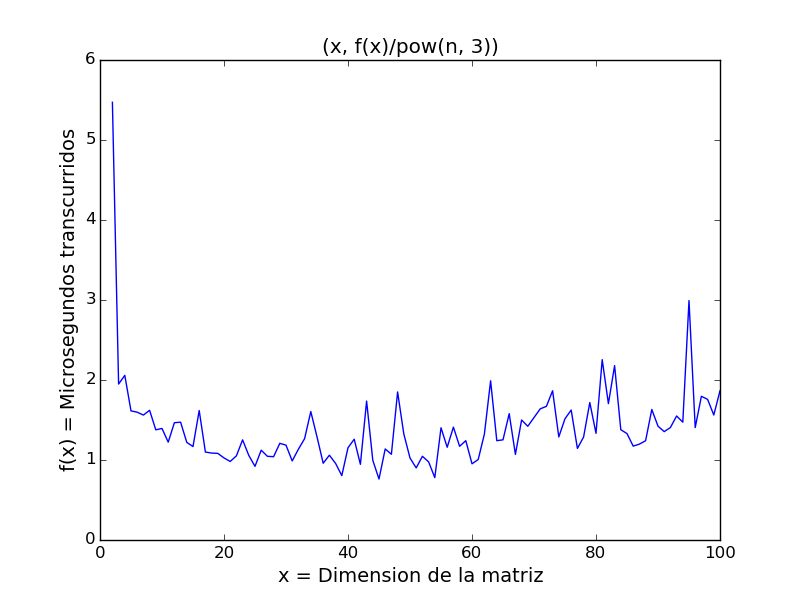
\includegraphics[scale=0.54]{images/4potenciasobrecubo}
\end{center}


\subsection{Mediciones de performance} \label{ej_3:performance}

\subsection{Conclusiones} \label{ej_3:conclusiones}

